
\chapter{Context}

\label{Context} 

% LC 43 References

%This chapter explains the current state of your topic, in practice and theory. This is the state of the world which you intend to improve, and the state of knowledge on top of which you build your advances and from which you learn knowledge to apply and constraints on your work. So, you will report and analyse what is known about a certain topic, as reported in reference literature and published scientific literature; if you are developing a product, you will need to report about comparable or competing products over which you intend to improve or from which you will obtain ideas; you may need to describe legal or societal situation within which your work takes place; etc.  
  
%It is important to demonstrate scholarship, i.e. the ability to read about a subject area in a range of sources, assimilate the material and then discuss it intelligently.  
  
%You should demonstrate that you understand what you have read by providing some analysis or commentary in view of the goals of your project: it is not enough simply to provide summaries of what you have read. References should be cited following the Harvard Referencing Style. You must also explain, both in this chapter and, as appropriate, in others, how the results of the studies to which you make reference inform your project work. To gain a passing grade, your report MUST demonstrate adequate engagement with academic literature and any other sources necessary for the work to be well informed.  

% The story we want to tell
% End to end learning - what does it mean
% Describe pipelined methods, contrast and compare to end to end methods

% Datasets and the importance of large public datasets for deep learning
% Synthetic datasets - how these become important as data can be difficult and costly to acquire

%% Prior methods used in image classification, using manual feature extraction

% What is end to end learning?
The properties of multilayer feedforward neural networks as universal function approximators has been studied extensively, especially in the 1980's . \cite{hornik1989multilayer} rigorously established that standard multilayer feedforward networks with as few as one hidden layer can approximate specific functions provided sufficiently many hidden units are available. while (\cite{cybenko1989approximation}) demonstrated analytically that a feedforward neural network with one hidden layer and any continuous sigmoidal nonlinearity can approximate any function with arbitrary precision providing that
no constraints are placed on the number of nodes or the size of the weights. As such, failures in applications can be attributed to inadequate learning, inadequate numbers of hidden units, or the presence of a  stochastic rather than a deterministic relation between input and target. (\cite{hornik1989multilayer}) state their results do not address the issue of how many units are needed to attain a  given degree of approximation.  
%% cybenko alternative entry
% backpropagation
Stochastic Gradient Descent (SGD) has become the standard for training deep neural networks
% training neural networks and the vanishing gradient problem

One of the main difficulties in training deep neural networks in the vanishing gradient problem, when, during the training phase, gradients become excessively large or small such that the network ceases to learn. This is also known as the degradation problem. 

\section{Related Work}
To be added, something surely must be happening in the field.
Work relating to digital noise:
Removing rain from images, vastly studied, i.e.
% https://arxiv.org/pdf/1909.08326.pdf
Adverse weather affecting sensor data including cameras used by AVs was surveyed by \cite{ZangAdverseWetherAVSurvey8666747}.  
\cite{ClearingSkiesDeepNNRainRemoval7893758}
\cite{Cord2014DetectingUR} "Advanced driver assistance systems (ADASs) based on video cameras are becoming pervasive in today's automotive industry. However, while most of these systems perform nicely in clear weather conditions, their performances fail drastically in adverse weather and particularly in the rain. We present two novel approaches that aim to detect unfocused raindrops on a car windshield using only images from an in-vehicle camera. Based on the photometric properties of raindrops, the algorithms rely on image processing techniques to highlight them. The results will be used to improve ADAS behavior under rainy conditions. Both approaches are compared with each other and the techniques from the literature."
\section{Quantifying noise}
\cite{yoneda2019automated} "There is a possibility that the recognition performance of the object is degraded due to the degradation of image quality. When installing a camera in the front of the vehicle, raindrops can be removed by installing the camera within the movable range of the wiper. However, when a camera is installed on the side or outside of the vehicle to capture images in all directions,the effects of raindrops are inevitable. Therefore, a camera installation that takes into account raindrops and a mechanism for removing them are necessary. In addition, researches on the recognition of rain-drops in the captured image have been reported".  
\cite{kurihata2005rainy} "We propose a weather recognition method from in-vehicle camera images that uses a
subspace method to judge rainy weather by detecting raindrops on the windshield."
Eigendrops" represent the principal components extracted from raindrop images in the
learning stage. Then the method detects raindrops by template matching. In experiments
using actual video sequences, our method showed good detection ability of raindrops and
promising results for rainfall judgment from detection results."  
  
 \cite{webster2015improved} "The presence of raindrop induced image distortion has a significant negative impact on the
performance of a wide range of all-weather visual sensing applications including within the
increasingly import contexts of visual surveillance and vehicle autonomy. A key part of this
problem is robust raindrop detection such that the potential for performance degradation in
effected image regions can be identified. Here we address the problem of raindrop detection
in colour video imagery using an extended feature descriptor comprising localised shape …"  
  
\cite{garg2007vision} "The visual effects of rain are complex. Rain produces sharp intensity changes in images and
videos that can severely impair the performance of outdoor vision systems. In this paper, we
provide a comprehensive analysis of the visual effects of rain and the various factors that …"  
  
\cite{garg2005does}

"Rain produces sharp intensity fluctuations in images and videos, which degrade the
performance of outdoor vision systems. These intensity fluctuations depend on various
factors, such as the camera parameters, the properties of rain, and the brightness of the …"

% on calculating light intensity of RGB value

% https://computergraphics.stackexchange.com/questions/5085/light-intensity-of-an-rgb-value

% on "smoothing" with matlab code provided:
% https://www.researchgate.net/profile/Manu_Bn2/publication/295235499_Rain_Removal_From_Still_Images_Using_L0_Gradient_Minimization_Technique/links/56c847aa08ae96cdd06acb6f.pdf

% Maybe a bit of history on SVM, HOG, SURF, etc. Perhaps best in introduction, like how this was a step, where manual feature extraction was used, then came end to end applied to computer vision problems.

% Intro explain term "end to end" - move to intro

% Context - successes in deep convolutional neural networks applied to computer vision problems

% 2. Imagenet - large public dataset \cite{deng2009imagenet}

%% MODELS

% 3. Alexnet - 
% 4. VGG - \cite{simonyan2015deep}
% 5. RESNET \cite{he2015deep}
% 6. Inception \cite{szegedy2014going}

% Then NVIDIA uses a deep convolutional neural networks architecture for end to end driving, i.e. image (raw pixels) in, vehicle control out.

% 1. NVIDIA end to end \cite{bojarski2016end}, DAVE2

% 7. \cite{Su_2019} 
% 8. \cite{zhang2017understanding}

%% However, these networks do have weaknesses, as demonstrated by \cite{Su_2019} in the form of one pixel attacks.
% \cite{zhang2017understanding} % demonstrated that simple depth two neural networks already have perfect finite sample expressivity as soon as the number of parameters exceeds the number of data points as it usually does in practice
%% Such examples question the robustness of deep convolutional neural networks. Especially in the context of one pixel attacks, when small addition of random noise causes the model to completely misinterpret the results, raising questions about generalisation, overfitting and robustness of the deep neural network architectures described.

%% DATASETS

%% 9. Audi dataset https://www.a2d2.audi/a2d2/en/download.html
% \cite{geyer2020a2d2},
%% 10. Ford Multi-AV Seasonal Dataset
% \cite{agarwal2020ford}
%% 11. Udacity
Maybe a bit on how synthetic datasets are used in other domains e.g. https://arxiv.org/pdf/1910.02550.pdf "ClearGrasp:
3D Shape Estimation of Transparent Objects for Manipulation" use of Blender. See section "Learning from synthetic data"

%% Identifying rainy data segments - Amazon Sagemaker 
% 19. \cite{joshi2020amazon}
% Mechanical Turk
% 20. \cite{crowston2012amazon}

%% SYNTHETIC DATASETS
% Cleargrasp
% 12. \cite{sajjan2019cleargrasp}

%% TOOLS -- maybe move tools to METHODS section
%% ROS
% \cite{quigley2009ros}

%% TENSORFLOW
% 13. \cite{abadi2016tensorflow}
%% KERAS
% 14. \cite{chollet2015keras}
%% PYTORCH
% 15. \cite{NEURIPS2019_9015}

% 3D environments
% 3D gaming engines
%% UNREAL - used by INTEL/AUDI/FORD TBC
% 16. \cite{unrealengine}
% user by AIRSIM
% 17. \cite{shah2017airsim}

%% UNITY - used by Udacity
% 18. \cite{haas2014history}

% Blender used to create synthetic datasets
% 21. \cite{rajpura2017object}

%% Public datasets
%Kaggle (\cite{kaggle_2020} contains over 50,000 public datasets and 400,000 public jupyter notebooks (\cite{JupyterNotebook2020}), an open-source web application that allows you to create and share documents that contain live code, equations, visualizations and narrative text. Uses include: data cleaning and transformation, numerical simulation, statistical modeling, data visualization and machine learning.

Imagenet is an example of the availability of a computer vision datasets. Public datasets exist for a number of tasks applied to computer vision, such as  
human action and activity recognition (\cite{chaquet2013survey}), agriculture (\cite{lu2020survey}) and hand pose estimation (\cite{li2019survey}).
Intel DevCloud (\cite{IntelDevCloud2020}).

%-----------------------------------
%	BACKGROUND
%-----------------------------------

% 
(Fig. \ref{fig:grigorescu-pipeline} as described by \cite{Grigorescu_2020} and \cite{Yurtsever_2020}

\begin{figure}[ht]
 \centering 
 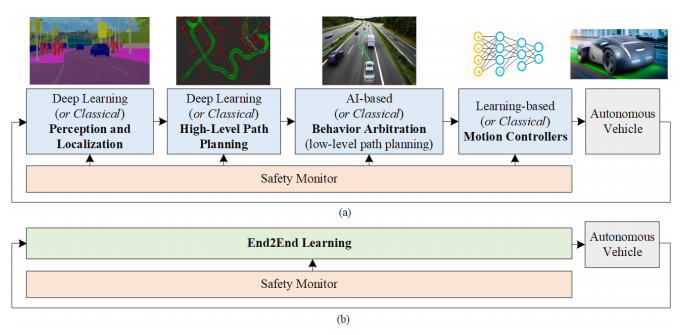
\includegraphics[scale=0.85]{Figures/grigorescu-pipeline.png}
 \caption{Diagrams showing the multisensor pipeline approach (a) and the end to end approach (b) as described by \cite{Grigorescu_2020}}
 \label{fig:grigorescu-pipeline}
\end{figure}


\begin{figure}[ht]
 \centering 
 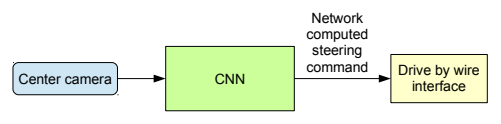
\includegraphics[scale=1]{Figures/bojarski-nvidia.png}
 \caption{Diagram of a trained network with a single centre camera input and a steering command output}
 \label{fig:bojarski-net}
\end{figure}

%% One pixel attacks

 (Fig. \ref{fig:one-pixel-attack}.
 
\begin{figure}[ht]
 \centering 
 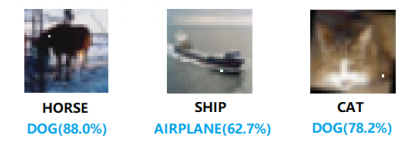
\includegraphics[scale=1]{Figures/one-pixel-attack.png}
 \caption{One-pixel  attacks  created  with the algorithm proposed by \cite{Su_2019} that  successfully  fooled  three  types  of deep neural networks trained  on  CIFAR-10 (\cite{CIFAR_10}) dataset. The modified pixel is white, the original  class  labels  are   black while  the  target  class  labels  and  the corresponding confidence are blue}
 \label{fig:one-pixel-attack}
\end{figure}

% fusion and end to end approach

(Fig. \ref{fig:grigorescu-pipeline} 

% bojarski
and training a CNN to map raw pixels from three front-facing camera directly to steering commands.



% A discussion of the proliferation of public datasets applied to machine learning, competitions, code repositiories, libraries is in order to contextualise the availability of data and tools in the context of our research

%-----------------------------------
%	End to End Learning
%-----------------------------------

\section{End to End Learning}

The  ImageNet Large-Scale Visual Recognition Challenge (ILSVRC) (Russakovsky et al., 2014) played an important part in the development of deep neural networks for image recognition. With the exception of DriveNet (NVIDIA end-to-end self-driving ConvNet architecture), all remaining four (AlexNet, GoogleLeNet, VGG and ResNet) were winning entries in the ILSVRC.  

% Interesting compact discussion on various applications of CCN and computer vision and end to end learning with several applications

% https://www.ncbi.nlm.nih.gov/pmc/articles/PMC6539483/ pg

%-----------------------------------
%	End to End Learning
%-----------------------------------

\section{Deep Learning applied to autonomous vehicles}

\subsection{Modular pipeline}

\subsection{End to end learning}



\lipsum[1]

%-----------------------------------
%	DATASETS
%-----------------------------------
\section{Datasets}

TODOS

\begin{itemize}
    \item Itemize / create table of datasets - see surveys
    \item Discuss importance of public datasets
    \item References
\end{itemize}

Advances in computer vision brought about by the Large Scale 
Explain:  
\begin{itemize}
    \item Convolution
    \item pre-processing
    \item Kernel/filter size
    \item Stride
    \item padding
    \item activation function
    \item Loss function
    \item optimisers
    \item Back-propagation
    % on this topic, a lot to cite, from Paul Werbos' PhD thesis "Beyond Regression: New Tools for Prediction and Analysis in the Behavioural Sciences, through Rummelhart et al. and LeCunn et al.
\end{itemize}

% contextualize data inbalance, make reference to methods.

